\chapter{Packages}
\label{ch:package}
\newenvironment{packclass}[0]{\textbf{Contained classes:} \begin{itemize}
}{\end{itemize}}
\newenvironment{packenum}[0]{\textbf{Contained enums:} \begin{itemize}
}{\end{itemize}}
\newenvironment{packif}[0]{\textbf{Contained interfaces:} \begin{itemize}
}{\end{itemize}}
\newenvironment{packpack}[0]{\textbf{Contained packages:} \begin{itemize}
}{\end{itemize}}
\newcommand{\packobj}[1]{\item #1}
\newcommand{\abstract}[1]{\textit{abstract} #1}

In this chapter, all packages and their purpose are introduced.

\section{MORR}

\begin{center}
    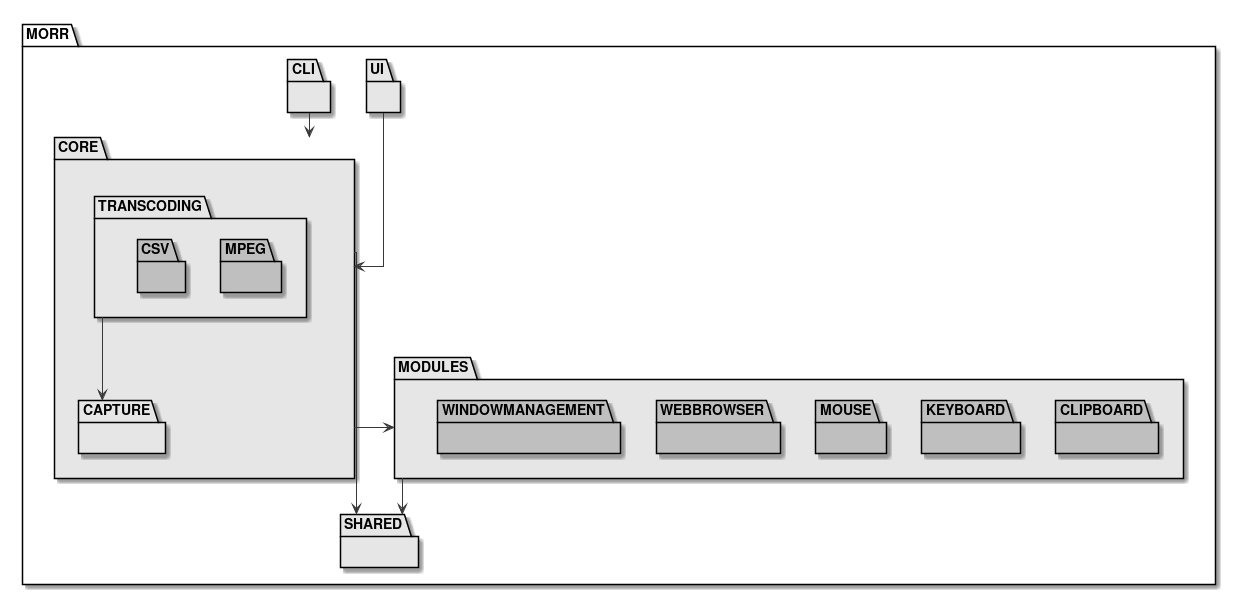
\includegraphics[width=1.0\textwidth]{resources/Packages/AllPackages.png}
\end{center}

The MORR package is the master package containing the whole application. It does not contain any classes directly as it only serves as a container for all packages required in the design.

\begin{packpack}
\packobj{CORE}
\packobj{CLI}
\packobj{SHARED}
\packobj{TRANSCODING}
\packobj{MODULES}
\packobj{UI}
\end{packpack}

\newpage
\section{MORR.CORE}

\begin{center}
    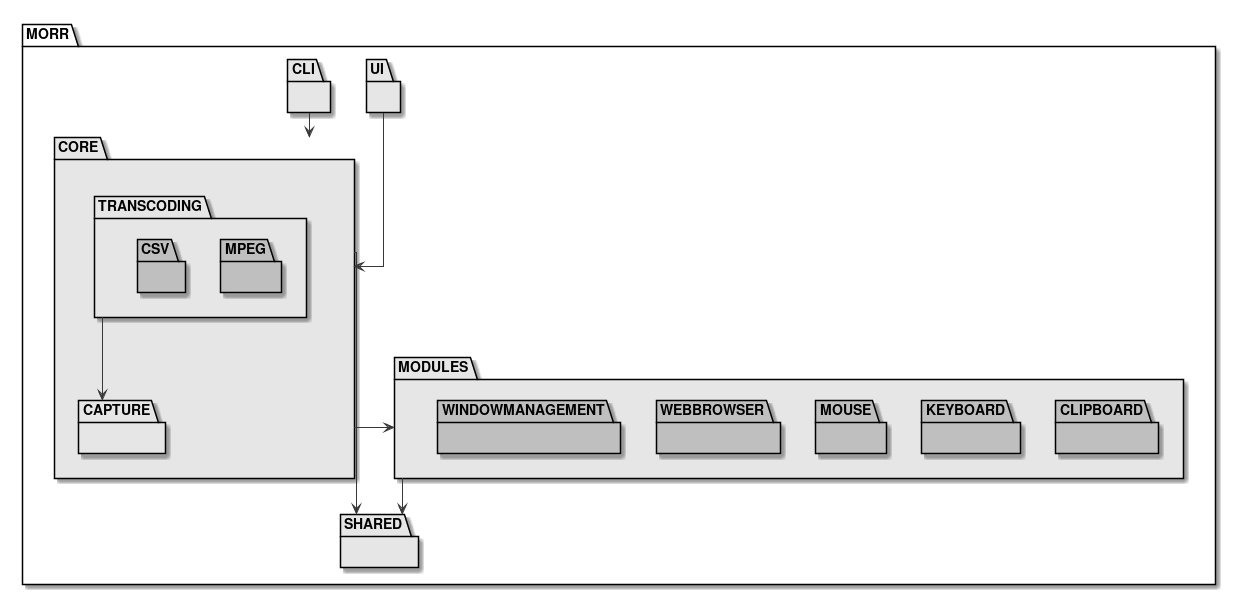
\includegraphics[width=1.0\textwidth]{resources/Packages/AllPackages.png}
\end{center}

The \textbf{CORE} package contains the central initializing logic to be called when the program is started and coordinates state-changes while the application is running.

\begin{packclass}
\packobj{RecordingManager}
\packobj{Bootstrapper}
\packobj{ModuleManager}
\packobj{ConfigurationManager}
\packobj{InvalidConfigurationException}
\end{packclass}

\begin{packif}
\packobj{IModuleManager}
\packobj{IBootstrapper}
\packobj{IConfigurationManager}
\packobj{IRecordingsManager}
\end{packif}

\newpage
\section{MORR.CLI}

\begin{center}
    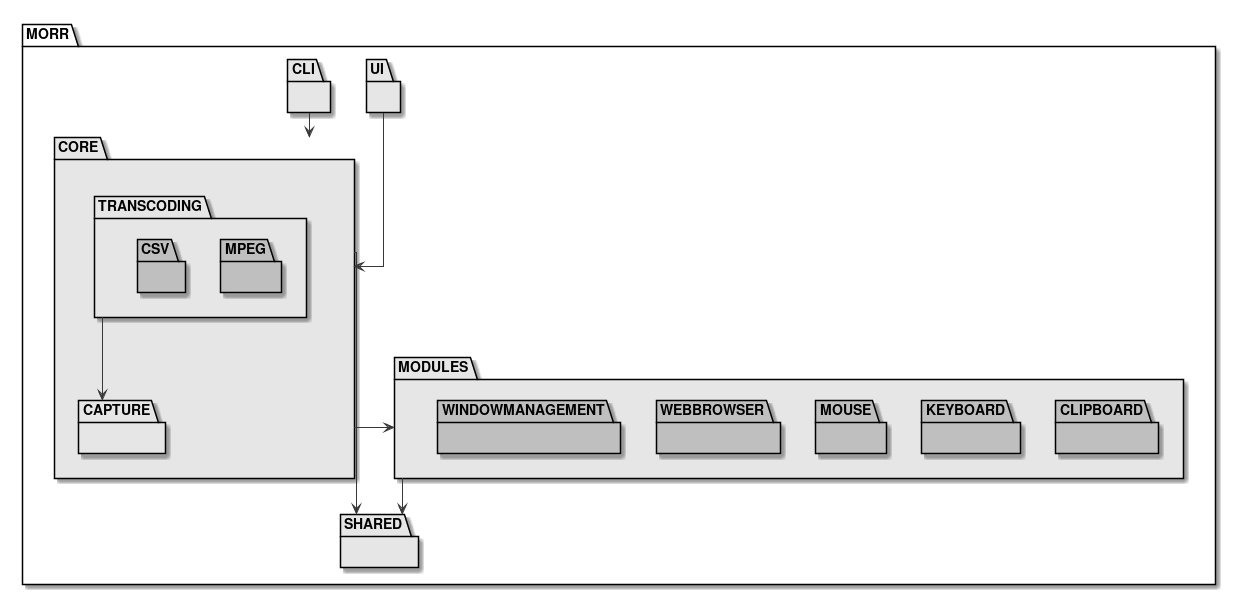
\includegraphics[width=1.0\textwidth]{resources/Packages/AllPackages.png}
\end{center}

The \textbf{CLI} package contains all logic exclusively needed for the command line interface which allows for the extraction of event data from saved recordings.

\begin{packclass}
\packobj{ProcessCommand}
\packobj{ProcessOptions}
\packobj{Executor}
\packobj{OutputFormatter}
\packobj{Options}
\packobj{Program}
\end{packclass}

\newpage
\section{MORR.SHARED}

\begin{center}
    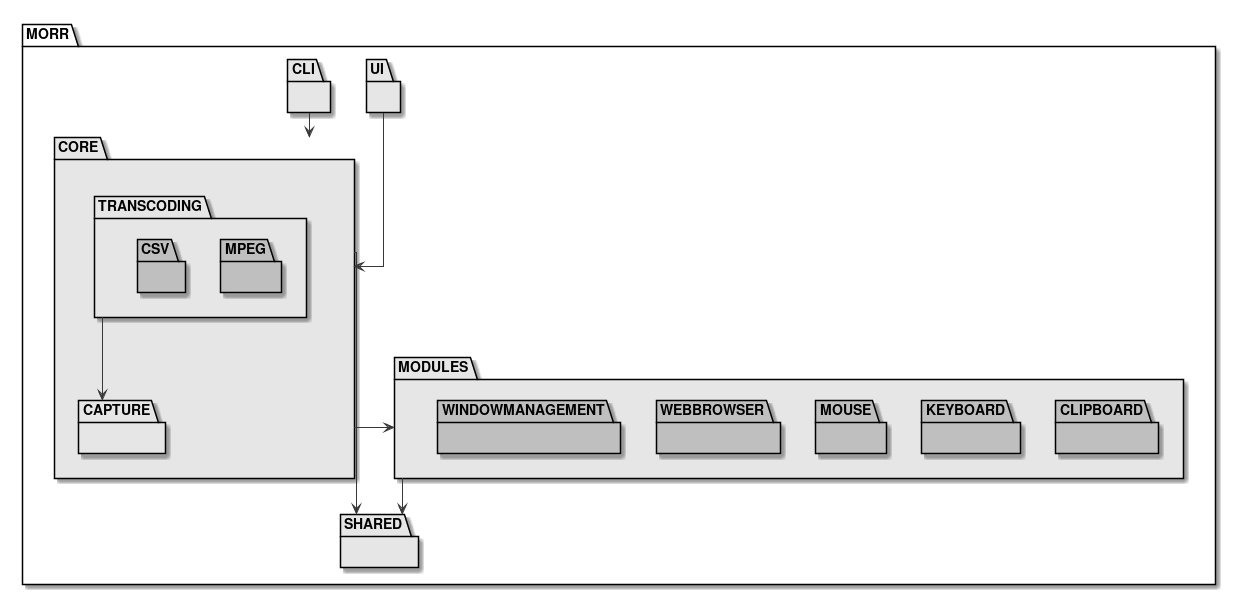
\includegraphics[width=1.0\textwidth]{resources/Packages/AllPackages.png}
\end{center}

The \textbf{SHARED} package provides interfaces and classes which have to be known and shared across multiple packages, such as the concept of an event or a module.

\begin{packif}
\packobj{IConfiguration}
\packobj{IModule}
\packobj{ITransformingModule}
\packobj{ICollectingModule}
\packobj{IReceivingModule}
\packobj{IReadOnlyEventQueue<out T>}
\packobj{IEventQueueStorageStrategy}
\end{packif}

\begin{packclass}
\packobj{\abstract{EventQueue<T>}}
\packobj{\abstract{Event}}
\packobj{RingBufferStorageStrategy<T>}
\packobj{RefCountedListStorageStrategy<T>}
\packobj{KeepAllStorageStrategy<T>}
\end{packclass}

\newpage
\section{MORR.TRANSCODING}

\begin{center}
    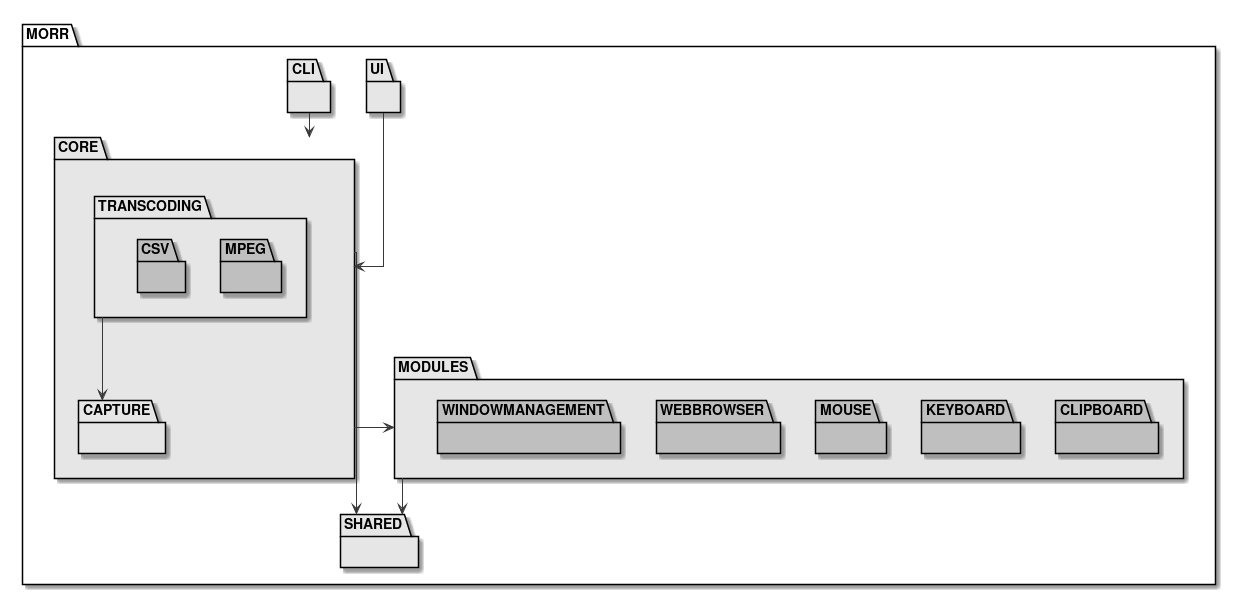
\includegraphics[width=1.0\textwidth]{resources/Packages/AllPackages.png}
\end{center}

The \textbf{TRANSCODING} package is responsible for serialization and deserialization of recorded video-, audio- and event-data. 

\begin{packif}
\packobj{IVideoCapture}
\packobj{IMetadataCapture}
\packobj{IDecoder}
\packobj{IEncoder}
\packobj{IMetaDataDeserializer}
\end{packif}

\begin{packclass}
\packobj{\abstract{VideoSample}}
\packobj{\abstract{MetadataSample}}
\packobj{DecodingException}
\packobj{EncodingException}
\packobj{CaptureException}
\packobj{MetadataDecodingException}
\packobj{VideoDecodingException}
\packobj{MetadataEncodingException}
\packobj{VideoEncodingException}
\packobj{VideoCaptureException}
\end{packclass}

\begin{packpack}
\packobj{CSV}
\packobj{MPEG}
\end{packpack}

\section*{MORR.TRANSCODING.CSV}
The \textbf{TRANSCODING.CSV} package is responsible for providing functionality which allows for encoding/decoding events from/to CSV (comma separated values) format.

\begin{packclass}
\packobj{CSVDecoder}
\packobj{CSVEncoder}
\end{packclass}

\section*{MORR.TRANSCODING.MPEG}
The \textbf{TRANSCODING.MPEG} package allows for storing video-, audio- and event-data in a MPEG container and also retrieving this data again from such a container.

\begin{packclass}
\packobj{MPEGEncoder}
\packobj{MPEGDecoder}
\packobj{DesktopCapture}
\packobj{<<static>> MonitorEnumerationHelper}
\packobj{<<static>> Durect3D11Helpers}
\packobj{<<static>> CaptureHelper}
\packobj{MonitorInfoEx}
\packobj{MonitorInfo}
\end{packclass}

\newpage
\section{MORR.MODULES}

\begin{center}
    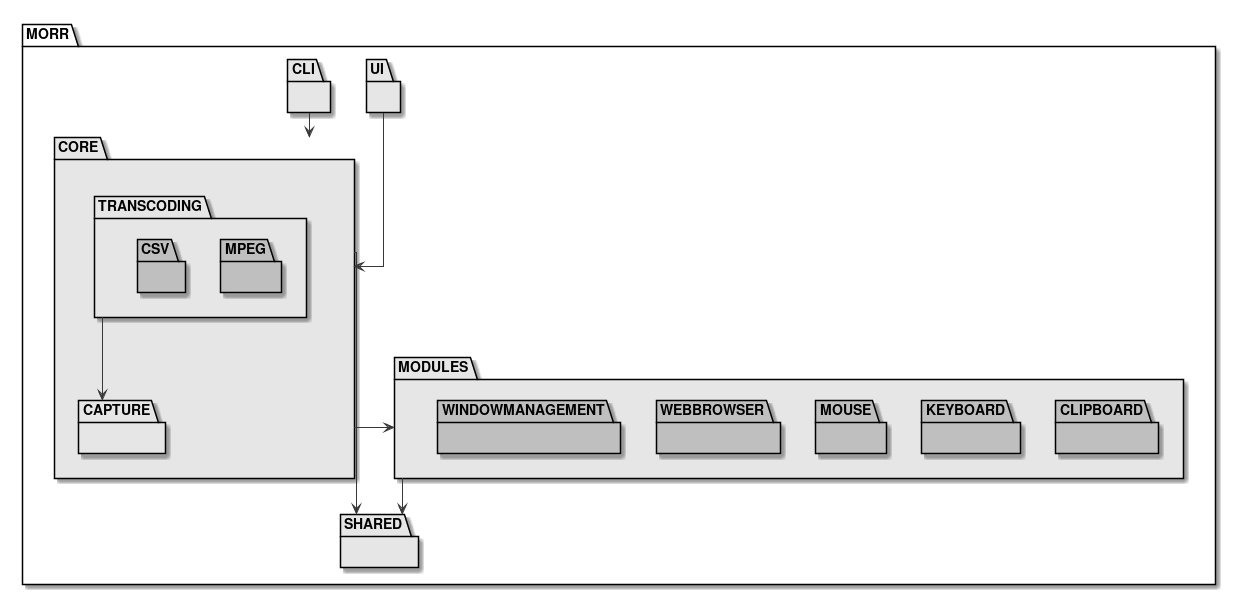
\includegraphics[width=1.0\textwidth]{resources/Packages/AllPackages.png}
\end{center}

The \textbf{MODULES} package serves as a container for all module-subpackages.

\begin{packpack}
\packobj{WINDOWMANAGEMENT}
\packobj{KEYBOARD}
\packobj{CLIPBOARD}
\packobj{WEBBROWSER}
\packobj{MOUSE}
\end{packpack}

\subsection*{MORR.MODULES.WINDOWMANAGEMENT}

\begin{center}
    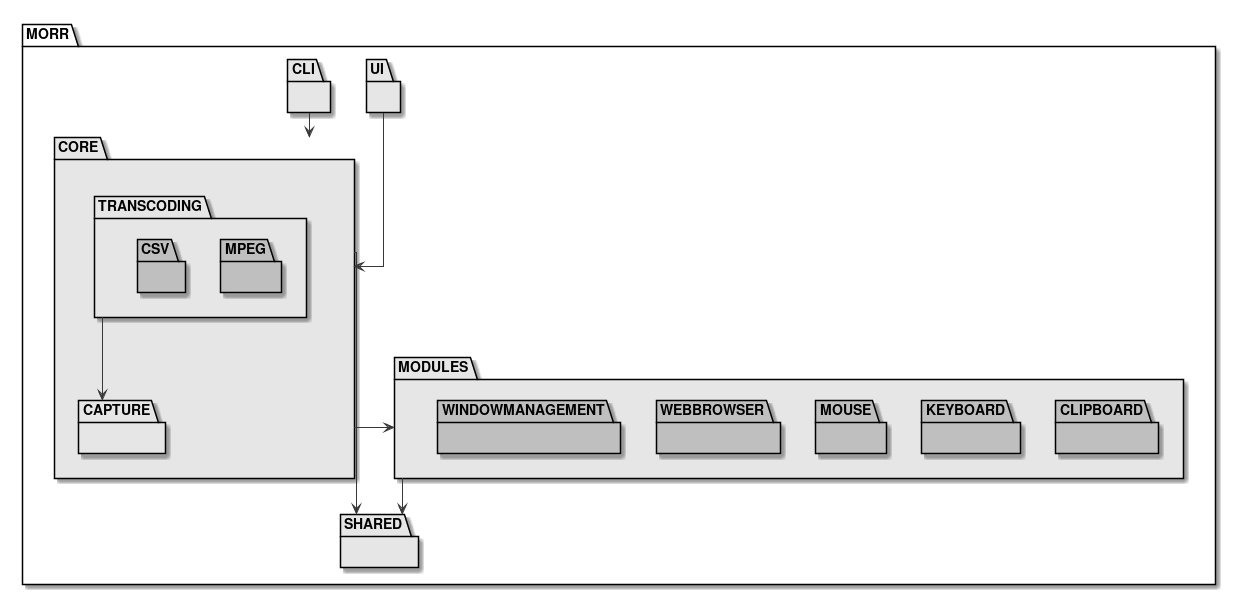
\includegraphics[width=1.0\textwidth]{resources/Packages/AllPackages.png}
\end{center}

The \textbf{WINDOWMANAGEMENT} package is responsible for providing the classes and concepts necessary for recording the window related user-interactions.

\begin{packclass}
\packobj{WindowManagementModule}
\packobj{\abstract{WindowEvent}}
\packobj{WindowMovementEvent}
\packobj{WindowFocusEvent}
\packobj{WindowSateChangedEvent}
\packobj{WindowResizingEvent}
\end{packclass}
\newpage
\subsection*{MORR.MODULES.KEYBOARD}

\begin{center}
    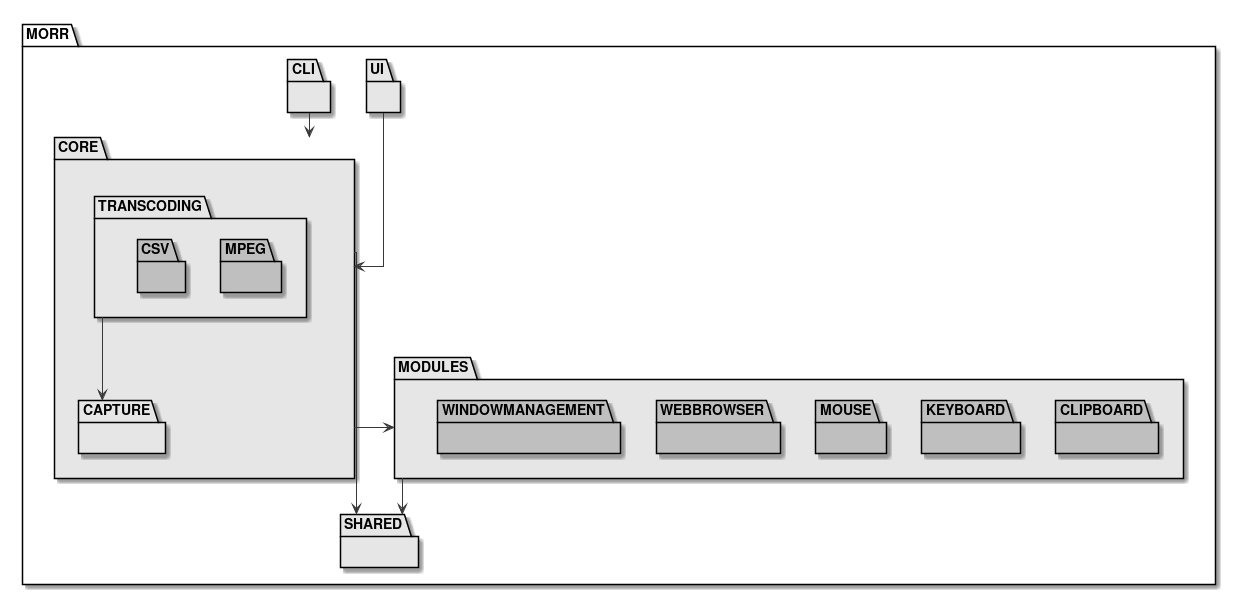
\includegraphics[width=1.0\textwidth]{resources/Packages/AllPackages.png}
\end{center}

The \textbf{KEYBOARD} package is responsible for providing the classes and concepts necessary for recording the keyboard related user-inputs.

\begin{packclass}
\packobj{\abstract{KeyboardEvent}}
\packobj{KeyboardModule}
\packobj{KeyboardInteractEvent}
\end{packclass}

\newpage
\subsection*{MORR.MODULES.WEBBROWSER}

\begin{center}
    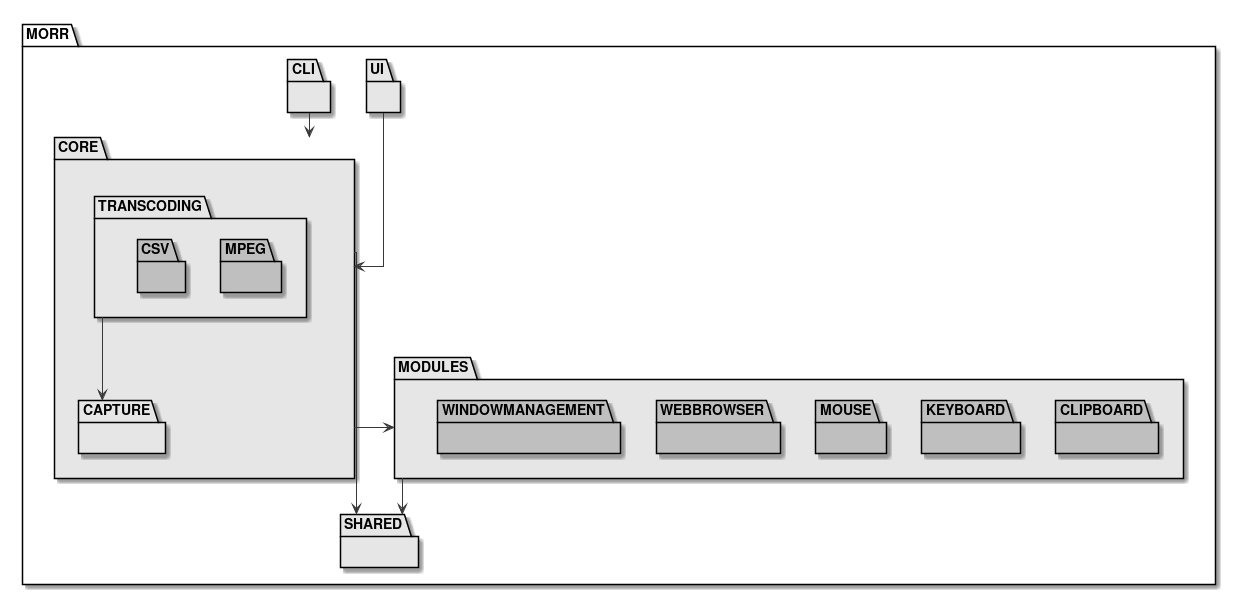
\includegraphics[width=1.0\textwidth]{resources/Packages/AllPackages.png}
\end{center}

The \textbf{WEBBROWSER} package is responsible for providing the classes and concepts necessary for recording the webbrowser related user-interactions.

\begin{packclass}
\packobj{WebBrowserModule}
\packobj{\abstract{WebBrowserEvent}}
\packobj{TextSelectionEvent}
\packobj{TextInputEvent}
\packobj{SwitchTabEvent}
\packobj{OpenTabEvent}
\packobj{CloseTabEvent}
\packobj{NavigationEvent}
\packobj{HoverEvent}
\packobj{FileDownloadEvent}
\packobj{ButtonClickEvent}
\end{packclass}

\newpage
\subsection*{MORR.MODULES.CLIPBOARD}

\begin{center}
    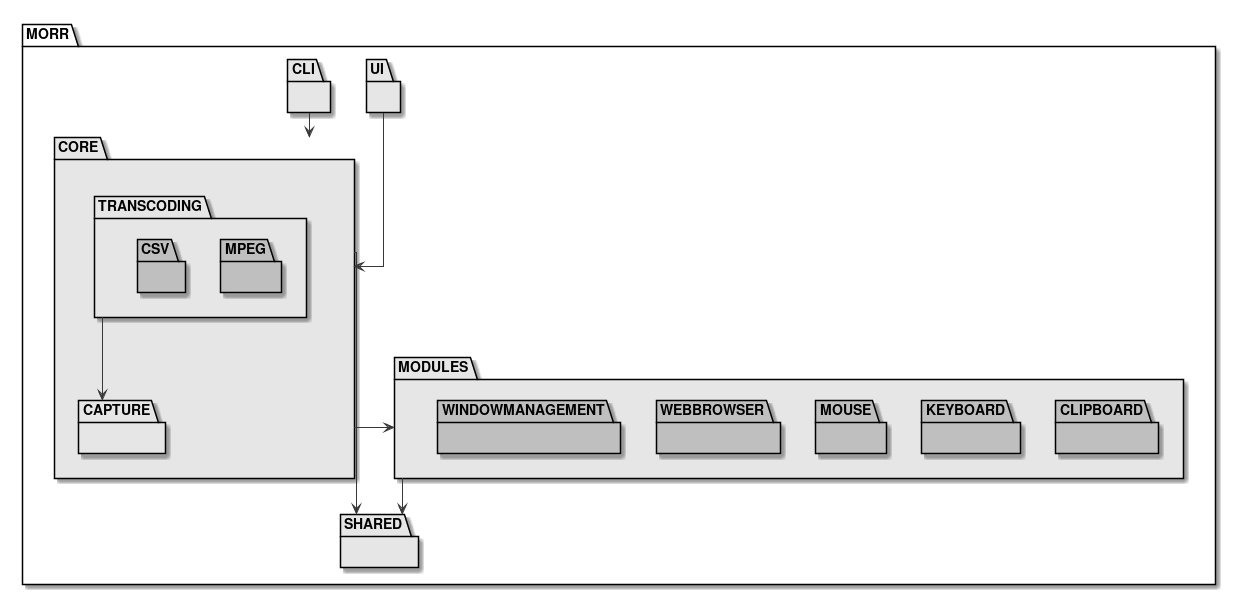
\includegraphics[width=1.0\textwidth]{resources/Packages/AllPackages.png}
\end{center}

The \textbf{CLIPBOARD} package is responsible for providing the classes and concepts necessary for recording the clipboard related user-interactions.

\begin{packclass}
\packobj{ClipboardModule}
\packobj{\abstract{ClipboardEvent}}
\packobj{ClipBoardInteractEvent}
\end{packclass}

\begin{packenum}
\packobj{InteractionType}
\end{packenum}

\newpage
\subsection*{MORR.MODULES.MOUSE}

\begin{center}
    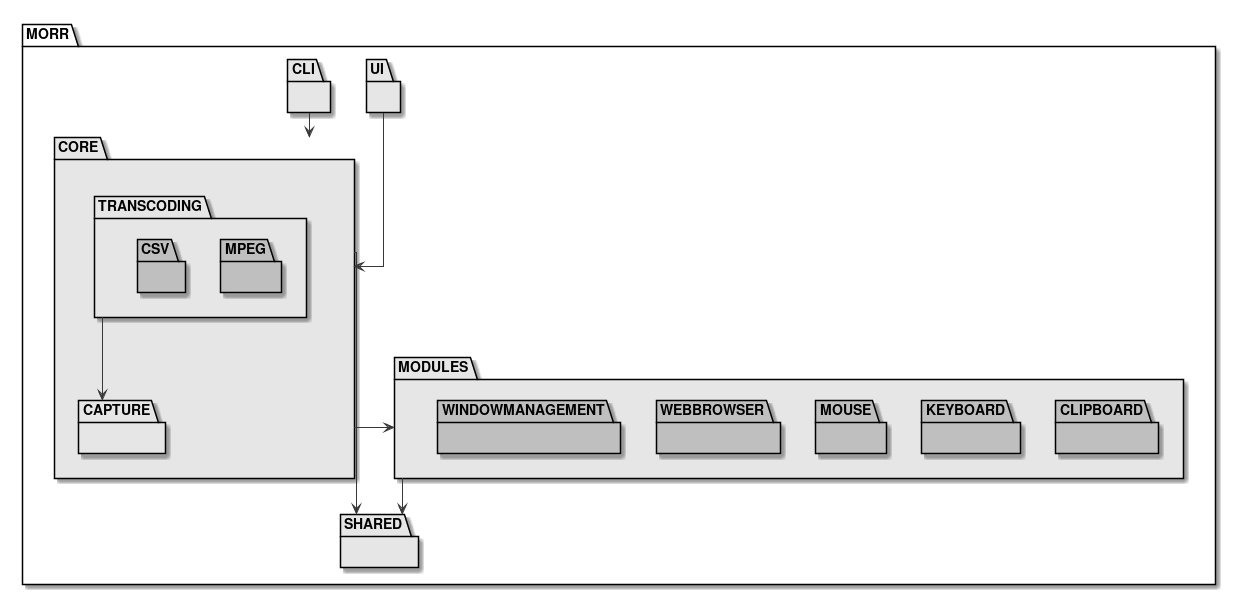
\includegraphics[width=1.0\textwidth]{resources/Packages/AllPackages.png}
\end{center}

The \textbf{MOUSE} package is responsible for providing the classes and concepts necessary for recording the mouse related user-inputs.

\begin{packclass}
\packobj{MouseModule}
\packobj{\abstract{MouseEvent}}
\packobj{MouseScrollEvent}
\packobj{MouseClickEvent}
\packobj{MouseMoveEvent}
\end{packclass}

\begin{packenum}
\packobj{MouseButton}
\packobj{MouseButtonState}
\end{packenum}
\newpage

\section{MORR.UI}

\begin{center}
    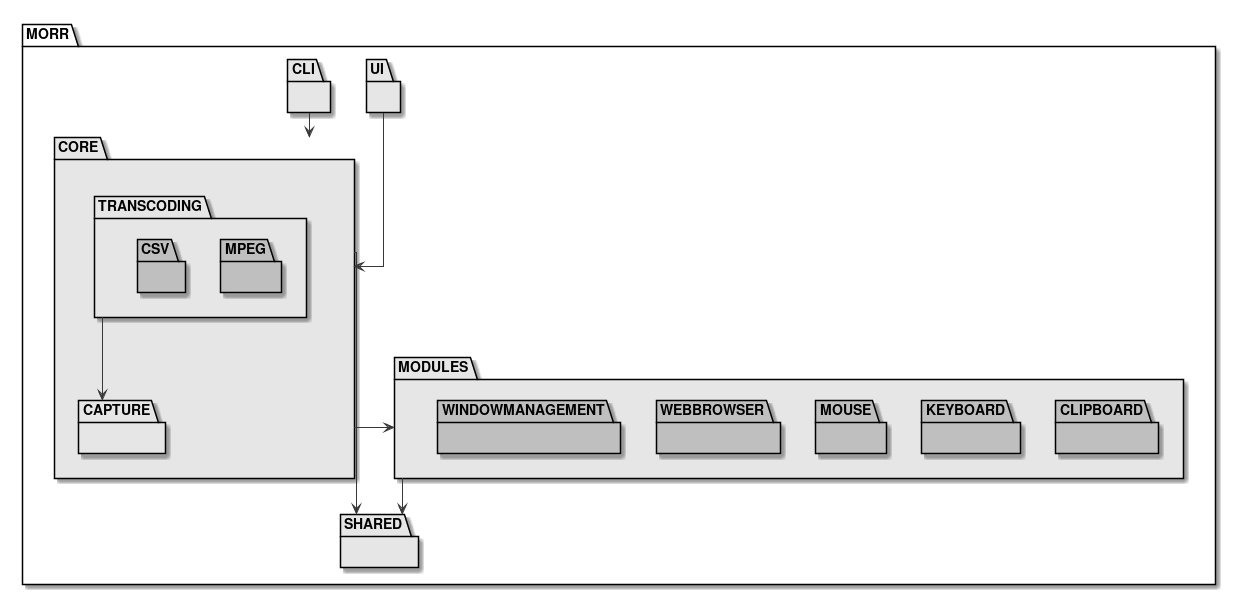
\includegraphics[width=1.0\textwidth]{resources/Packages/AllPackages.png}
\end{center}

The \textbf{UI} package is responsible for the graphical user interface.

\begin{packif}
\packobj{ICommand}
\end{packif}

\begin{packclass}
\packobj{ContextMenu}
\packobj{NotifyIcon}
\packobj{<<partial> App}
\packobj{ImageSource}
\packobj{<<partial>> InformationDialog}
\packobj{<<partial>> SaveDialog}
\packobj{<<partial>> ErrorDialog}
\packobj{ApplicationViewModel}
\packobj{RelayCommand}
\end{packclass}
